\section{Ragionamento probabilistico e Bayesian Network}\

\noindent Il ragionamento probabilistico è una forma di ragionamento che sfrutta la teoria della
probabilità, in particolar modo dipendenza e indipendenza tra variabili e regola di
Bayes. Nel ragionamento probabilistico si assegnano probabilità a ipotesi ed eventi e
si utilizzano le probabilità a posteriori per i ragionamenti. Un’applicazione del
ragionamento probabilistico sono le reti bayesiane. Queste vengono rappresentate
mediante grafi orientati aciclici (DAG) dove ogni nodo del grafo rappresenta una
variabile e gli archi indicano le dipendenze probabilistiche tra le variabili.

\subsection{Apprendimento della struttura}
\noindent Date le risorse ocmputazionali a disposizione, si è sfruttata la \textit{feature importance} emersa dagli esperimenti precedenti per selezionare le variabili da mantenere per apprendere la struttura della rete bayesiana.
Le feature che verranno utilizzate sono le seguenti: \textit{Rating Agency, Rating, Sector, Current Ratio, Debt/Equity Ratio, Gross Margin, EBITDA Margin, Net Profit Margin, Asset Turnover, ROI - Return On Investment, Operating Cash Flow Per Share}.
\\ I valori continui sono stati discretizzati mediate \textit{KBinsDiscretizer}, la struttura è stata appresa mdiante l'utilizzo dell'\textit{HillClimbSearch} e come \textit{estimator} la \textit{Maximum Likelihood Estimator}. 
\\ Di seguito si riporta la struttura della rete:
\begin{figure}[H]
    \centering
    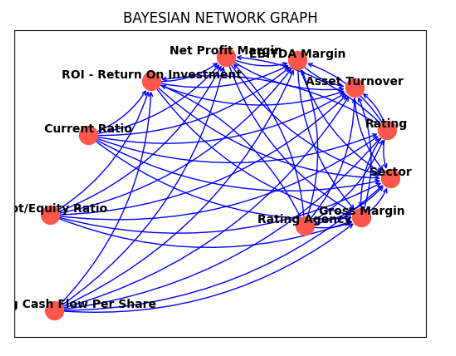
\includegraphics[scale=0.8]{img/bn.png}
\end{figure}
\noindent Di seguito si riporta l'esempio di una \textit{CPD}:

\begin{figure}[H]
    \centering
    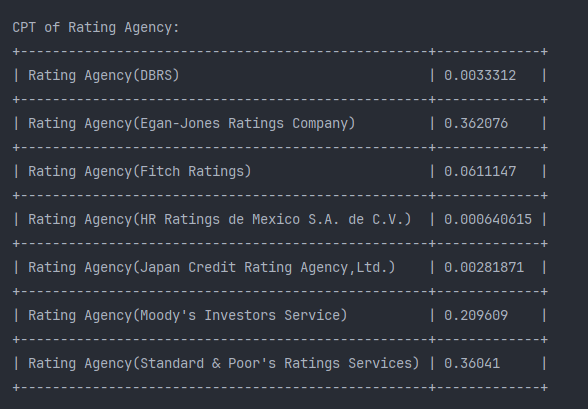
\includegraphics[scale=0.6]{img/cpt.png}
\end{figure}

\subsection{Generazione di sample}
\noindent Tramite la rete bayesiana è possibile generare nuovi sample, ovvero nuove configurazioni di variabili. Questo è utile per generare nuovi dati da utilizzare per addestrare un modello, o per fare inferenza su nuovi dati. 

% TODO: inserire screen di esempio

\subsection{Gestione di dati mancanti}

\noindent Le reti bayesiane sono in grado di gestire casi in cui una variabile di input non è nota. Questo è utile in quanto i dati reali spesso presentano valori mancanti. La rete bayesiana è in grado di fare inferenza su nuovi dati, anche se non tutte le variabili sono note.

% TODO: inserire screen di esempio

\subsection{Query di esempio}
\noindent Le reti bayesiane sono in grado di rispondere a query probabilistiche, ovvero di calcolare la probabilità di una variabile dato un insieme di evidenze. Di seguito si riporta un esempio di query:
\begin{itemize}[label=-]
    \item \textbf{Query}: Qual è la probabilità che una società abbia un rating "AAA" (Rischio basso) dato che il suo \textit{Current Ratio} è 1.5 e il suo \textit{Debt/Equity Ratio} è 0.5?
\end{itemize}